% Chapter on Distributed Deep Learning.
%
% Developed for my Master Thesis at Maastricht University.
% Based on Eugenio Senes's template at the University of Torino.
%
% By Joeri Hermans (joeri@joerihermans.com)
%
% Released under an MIT license. Share, modify and enjoy, but quote the author!

\chapter{Distributed Deep Learning}
\label{chapter:distributed_deep_learning}

In this chapter, we introduce several concepts and techniques related to Distributed Deep Learning on which this works builts upon. We start in Section~\ref{sec:ddl_introduction} with a recap of all methods and techniques we have discussed in Chapter~\ref{chapter:introduction}. Afterwards, we continue with a discussion of synchronous followed by an examination of asynchronous optimization methods such as \textsc{downpour} and closely related extensions. Furthermore, we address several issues such as \emph{asynchrony induced momentum} which are related to asynchronous optimization. We also consider several approaches which provide a possible solution to these issues.

\section{Introduction}
\label{sec:ddl_introduction}

For all practical applications, Stochastic Gradient Descent (\textsc{sgd}) and derrivatives are the best tools from the numerical optimization toolbox for neural networks. However, applying \textsc{sgd} in its pure form, that is, updating the parameters after evaluating a training sample, is a computationally intensive process. An initial approach for speeding up \textsc{sgd} in terms of convergence with respect to training time was to compute the gradients of several samples, a \emph{mini-batch}, and average them. This approach has several advantages, the first being that a larger mini-batch will result in less noisy updates, as more ``evidence'' of the surrounding error space will provide a better gradient update. The second advantage being the increased computational parallelism, since all sub-gradients (gradients of the training samples in the mini-batch) are based upon the same parametrization of the model. As a result, the parallelization of the gradient computation is quite straightforward. For instance, for every training sample in a mini-batch, one could allocate a thread, a process, or even a different machine (see Figure~\ref{fig:distributed_mini_batch_parallelism}) to compute the gradients in parallel. However, a blocking mechanism is required in order to sum all gradients, average them, and finally update the parametrization of the model. This process is depicted in Figure~\ref{fig:minibatch_data_parallelism}. As discussed in Chapter~\ref{chapter:introduction}, mini-batch parallelism is an instance of \emph{synchronous data parallelism}. Although many synchronous optimization schemes share a similar structure, we discuss other instances of synchronous data parallelism in particular in Section~\ref{sec:synchronous_data_parallelism} since these optimization schemes incorperate gradients and worker parameterizations into the central variable differently compared to mini-batch parallelism.\\

Nevertheless, a significant, but albeit technical issue in synchronous optimization is when a single or multiple workers are slowed down for some reason, e.g., due to high CPU load, or bandwidth consumption, other workers will have to wait before they can continue with step $t + 1$. As a result, the allocated resources are not fully utilized. This particular issue is known in literature as the \emph{straggler} problem. However, this problem can be mitigated with by using a \emph{homogeneous} hardware configuration. For instance, when one would employ 2 different GPU's running at different clock speeds, a \emph{heteregenous} hardware configuration, then the CPU will always have to wait for a particulur GPU since it runs at a lower clock speed causing the complete training procedure to be slowed down\footnote{A chain is only as strong as its weakest link.}. Furthermore, we could argue that there is a limit to synchronous data parallelism because simply \emph{adding more workers to the problem implicitly increases the size of the mini-batch}. As a result, when applying synchronous data parallelism, one is not parallelizing gradient descent in the typical sense, but rather parallelizing the computations within a step. Of course, one could even increase the parallelism within synchronous data parallelism even further by applying model parallelism as dicussed briefly in Section~\ref{sec:intro_model_parallelism}. Nevertheless, while such an implementation is definitly possible, it might be more cost-aware from an economical perspective to just let the model train for a longer period of the compared to actually implementing the training procedure described above. Furthermore, even with if one would implement said training method, there is still a limit to the amount parallelism due to the structure of the computation graph, and communication cost between devices which have to be taken into account. This of course begs the question if it is actually possible to push the limits of asynchrony, and thereby reducing the training time even further. Or from a different perspective, is there a more trivial method besides implementing the above training procedure to reduce the training time.\\

Several approaches~\cite{dean2012large, ho2013more, cipar2013solving, recht2011hogwild, zhang2015deep, louppe2010zealous, jiang2017heterogeneity} have been suggested over the past years which accomplish exactly this. All these methods are instances of \emph{asynchronous data parallelism}, discussed in Section~\ref{sec:intro_data_parallelism}. In contrast to synchronous data parallelism, asynchronous methods can be identified by the \emph{absence} of a blocking mechanism which is present in synchronous data parallelism. Despite the fact that this method resolves the waiting time induced by stragglers, it introduces a closely related but persistent issue. More formally, the \emph{staleness} issue is due to the fact that all $n$ workers update the central variable in an asynchronous fashion. Meaning, from the moment a worker $k$ is done computing an update $\Delta\theta^k$ based upon parameterization of the central variable $\tilde{\theta}_{t}$, it will commit $\Delta\theta^k$ to the parameter server, and afterwards continue with the next mini-batch. Because of this behaviour, it is possible that a number of central variable updates $\tau$ occurred during the time worker $k$ was computing $\Delta\theta^k$. As a result, instead of obtaining $\tilde{\theta}_{t+1}$ by applying $\Delta\theta^k$, worker $k$ is actually applying $\Delta\theta^k$ to $\tilde{\theta}_{t+\tau}$. Which is not ideal, since $\Delta\theta^k$ is based on parametrization $\tilde{\theta}_t$. From~\cite{implicitmomentum} we know that increasing the number of workers actually increases the amount of staleness $\tau$ since $\mathbf{E}[\tau] = (n - 1)$ under a \emph{homogeneous} hardware configuration and a simple queuing model\footnote{With a simple queuing model we intent that updates $\Delta\theta^k$ are incorperated into the central variable in a queuing fashion.}. This result is validated empirically in one of our experiments, shown in Figure~\ref{fig:staleness_distribution}.

\begin{figure}[h]
  \centering
  \begin{subfigure}{.45\textwidth}
    \centering
    \includegraphics[width=\linewidth]{resources/images/staleness_10}
    \caption{$n = 10$}
    \label{fig:staleness_distribution_10}
  \end{subfigure}
  \begin{subfigure}{.45\textwidth}
     \centering
     \includegraphics[width=\linewidth]{resources/images/staleness_20}
     \caption{$n = 20$}
    \label{fig:staleness_distribution_20}
  \end{subfigure}
  \begin{subfigure}{.45\textwidth}
     \centering
     \includegraphics[width=\linewidth]{resources/images/staleness_30}
     \caption{$n = 30$}
     \label{fig:staleness_distribution_30}
  \end{subfigure}
  \caption{These figures show the staleness distribution during a training procedure using a differing number of parallel workers. For every central variable update, we record the staleness $\tau$, and increment the number of occurences of this particular staleness by 1. Thus effectievely building a histogram showing the staleness distribution during the training. With this, we experimentally validate the observations of~\cite{implicitmomentum} that $\mathbf{E}[\tau] = (n - 1)$. Furthermore, the claim that staleness is geometrically distributed during training also holds (right half of the distribution).}
  \label{fig:staleness_distribution}
\end{figure}

\section{Synchronous Data Parallelism}
\label{sec:synchronous_data_parallelism}

\subsection{Model Averaging}
\label{sec:model_averaging}

\begin{figure}[H]
  \centering
  %% 1
  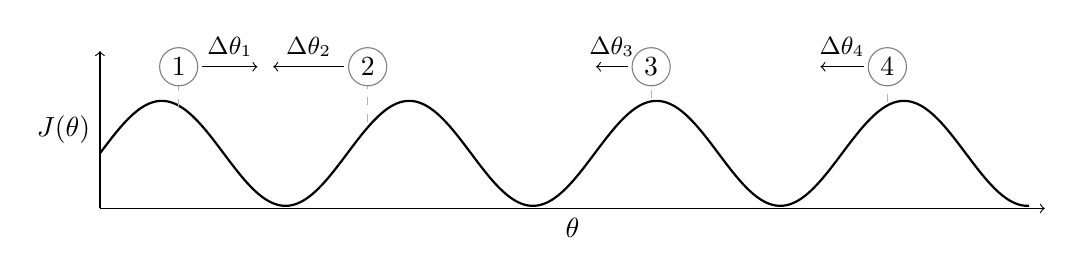
\begin{tikzpicture}
    % Draw the axis of the plots.
    \draw[->] (0,0) -- (12,0) node[midway, below] {$\theta$};
    \draw[->] (0,0) -- (0, 2) node[midway, left] {$J(\theta)$};
    % Draw the hypothesis space, which is sin(x) / 2 + 0.55
    \draw[samples=400,domain=0:11.8,smooth,variable=\x,black,thick]  plot ({\x},{sin(deg(\x * 2)) / 1.5 + 0.7});
    % Draw the instances, and their gradient arrows.
    \draw (1,1.8) node[circle,inner sep=2pt,draw=black!50] {1};
    \draw[dashed, draw=black!30] (1,1.28) -- (1,1.55);
    \draw[->] (1.3,1.8) -- (2,1.8) node[midway, above] {\small $\Delta\theta_1$};

    \draw (3.4,1.8) node[circle,inner sep=2pt,draw=black!50] {2};
    \draw[dashed, draw=black!30] (3.4,1.1) -- (3.4,1.55);
    \draw[->] (3.1,1.8) -- (2.2,1.8) node[midway, above] {\small $\Delta\theta_2$};

    \draw (7,1.8) node[circle,inner sep=2pt,draw=black!50] {3};
    \draw[dashed, draw=black!30] (7,1.4) -- (7,1.55);
    \draw[->] (6.7,1.8) -- (6.3,1.8) node[midway, above] {\small $\Delta\theta_3$};

    \draw (10,1.8) node[circle,inner sep=2pt,draw=black!50] {4};
    \draw[dashed, draw=black!30] (10,1.35) -- (10,1.55);
    \draw[->] (9.7,1.8) -- (9.15,1.8) node[midway, above] {\small $\Delta\theta_4$};
  \end{tikzpicture}
  %% 2
  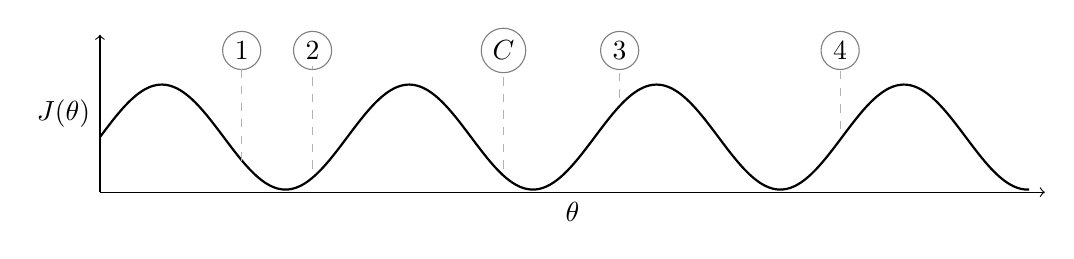
\begin{tikzpicture}
    % Draw the axis of the plots.
    \draw[->] (0,0) -- (12,0) node[midway, below] {$\theta$};
    \draw[->] (0,0) -- (0, 2) node[midway, left] {$J(\theta)$};
    % Draw the hypothesis space, which is sin(x) / 2 + 0.55
    \draw[samples=400,domain=0:11.8,smooth,variable=\x,black,thick]  plot ({\x},{sin(deg(\x * 2)) / 1.5 + 0.7});
    % Draw the instances, and their gradient arrows.
    \draw (1.8,1.8) node[circle,inner sep=2pt,draw=black!50] {1};
    \draw[dashed, draw=black!30] (1.8,0.4) -- (1.8,1.6);

    \draw (2.7,1.8) node[circle,inner sep=2pt,draw=black!50] {2};
    \draw[dashed, draw=black!30] (2.7,0.3) -- (2.7,1.6);

    \draw (6.6,1.8) node[circle,inner sep=2pt,draw=black!50] {3};
    \draw[dashed, draw=black!30] (6.6,1.2) -- (6.6,1.6);

    \draw (9.4,1.8) node[circle,inner sep=2pt,draw=black!50] {4};
    \draw[dashed, draw=black!30] (9.4,0.8) -- (9.4,1.6);
    % Draw the center variable.
    \draw (5.125,1.8) node[circle,inner sep=2pt, draw=black!50] {$C$};
    \draw[dashed, draw=black!30] (5.125,0.3) -- (5.125,1.5);
  \end{tikzpicture}
  %% 3
  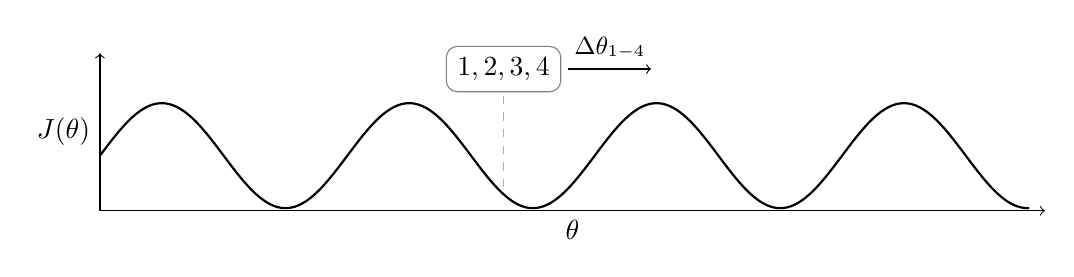
\begin{tikzpicture}
    % Draw the axis of the plots.
    \draw[->] (0,0) -- (12,0) node[midway, below] {$\theta$};
    \draw[->] (0,0) -- (0, 2) node[midway, left] {$J(\theta)$};
    % Draw the hypothesis space, which is sin(x) / 2 + 0.55
    \draw[samples=400,domain=0:11.8,smooth,variable=\x,black,thick]  plot ({\x},{sin(deg(\x * 2)) / 1.5 + 0.7});
    % Draw the instances, and their gradient arrows.
    \draw (5.125,1.8) node[rectangle,rounded corners,inner sep=4pt, draw=black!50] {$1,2,3,4$};
    \draw[dashed, draw=black!30] (5.125,0.3) -- (5.125,1.5);
    \draw[->] (5.95,1.8) -- (7,1.8) node[midway, above] {\small $\Delta\theta_{1-4}$};
  \end{tikzpicture}
  \caption{Caption here}
\end{figure}

\subsection{Elastic Averaging SGD}
\label{sec:easgd}

\begin{figure}[H]
  \centering
  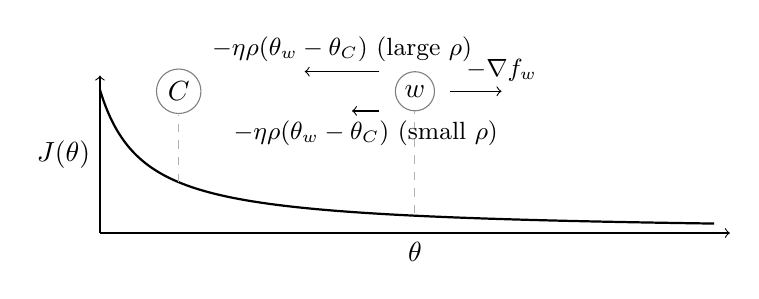
\begin{tikzpicture}
    % Draw the axis of the plots.
    \draw[->] (1,0) -- (9,0) node[midway, below] {$\theta$};
    \draw[->] (1,0) -- (1,2) node[midway, left] {$J(\theta)$};
    % Draw the function.
    \draw[samples=400,domain=1:8.8,smooth,variable=\x,black,thick]  plot ({\x},{(1 / (\x - 0.45))});
    % Draw the instances (including the center variable) with the gradient arrows and the elastic difference.
    \draw (2, 1.8) node[circle, inner sep=2pt, draw=black!50] {$C$};
    \draw[dashed, draw=black!30] (2,0.65) -- (2,1.5);
    \draw (5, 1.8) node[circle, inner sep=2pt, draw=black!50] {$w$};
    \draw[dashed, draw=black!30] (5,0.25) -- (5,1.55);
    % Draw the gradients and the elastic force.
    \draw[->] (5.45,1.8) -- (6.1,1.8) node[right, above] {\small $-\nabla f_w$};
    \draw[->] (4.55,1.55) -- (4.2,1.55) node[midway, below] {\small $-\eta\rho(\theta_w - \theta_C)$ (small $\rho$)};
    \draw[->] (4.55,2.05) -- (3.6,2.05) node[midway, above] {\small $-\eta\rho(\theta_w - \theta_C)$ (large $\rho$)};
  \end{tikzpicture}
  \caption{EASGD Caption here}
\end{figure}

\section{Asynchronous Data Parallelism}
\label{sec:asynchronous_data_parallelism}

\subsection{DOWNPOUR}
\label{sec:downpour}

\subsection{Dynamic SGD}
\label{sec:dyn_sgd}

\subsection{Asychrony Induced Momentum}
\label{sec:implicit_momentum}

\subsection{Asynchronous Elastic Averaging SGD}
\label{sec:aeasgd}

\section{Hybrids}
\label{sec:hybrids}
